\documentclass[dm,ppgcomp]{texfurg} %ppgmc ou ppgcomp

\usepackage[utf8]{inputenc} % acentuacao
\usepackage[T1]{fontenc}

\usepackage{graphicx} % para inserir figuras
\usepackage{amsmath}
\usepackage{multirow}
\usepackage{ amssymb }
\usepackage{ wasysym }
\usepackage{ upgreek }
\usepackage{pifont}
\usepackage{amssymb}
\newcommand{\cmark}{\ding{51}}%
\newcommand{\xmark}{\ding{55}}%
\usepackage{subfigure}
\usepackage[section]{placeins} % sometimes useful to prevent figures from floating out of a section
\usepackage{ tipa }
\usepackage{cancel}
\usepackage{booktabs}
\usepackage[flushleft]{threeparttable} % Adicionar notas em tabelas
\renewcommand{\arraystretch}{1.2} % Aumenta o tamanho do espaço entre linhas


\title{Qualificação}

\author{Rodrigues}{Bruno Coelho}
\advisor[Prof.~Dr.]{Gonçalves}{Eder Mateus}
%\coadvisor[Prof.~Dr.]{Aguiar}{Marilton Sanchotene de}
%\collaborator[Prof.~Dr.]{Aguiar}{Marilton Sanchotene de}

\examiner{Prof.~Dr.~Armando Multas}
\examiner{Prof\textsuperscript{a}.~Dr\textsuperscript{a}.~Nomelinda Longuinha da Silva Paes Netto}
\examiner{Prof.~MSc.~Gerúndio das Dores}

\keyword{palavrachave-um}
\keyword{palavrachave-dois}
\keyword{palavrachave-tres}
\keyword{palavrachave-quatro}

\begin{document}

%\renewcommand{\advisorname}{Orientadora}           %descomente caso tenhas orientadora
%\renewcommand{\coadvisorname}{Co-orientadora}      %descomente caso tenhas co-orientadora

\maketitle

\sloppy

%Sumario
\tableofcontents

\chapter{Introdução}
  

\section{Objetivos}


 
\section{Motivação e Justificativa}


\section{Metodologia}



\section{Organização do Trabalho}



\chapter{Referencial Teórico/ Revisão Bibliográfica}

\section{Teste de Software}

O teste faz parte de um método de verificação e validação de software onde a verificação investiga se o software atende aos seus requisitos funcionais e não funcionais enquanto a validação é um processo mais amplo no qual o objetivo é garantir que o software atenda às expectativas do cliente, sendo essencial já que nem sempre as especificações dos requisitos refletem os desejos ou necessidades reais dos clientes e usuários do sistema \cite{sommerville2010}. O termo garantir refere-se ao processo que visa obter confiança de que um sistema se comportará adequadamente \cite{winikoff2010assurance}. 

O processo de verificação e validação possuem outras atividades além dos testes, entre elas as inspeções e revisões de software. Estas atividades analisam e verificam os requisitos do sistema, os modelos de projeto, o código-fonte do programa e os testes propostos para o sistema Figura \ref{fig:ver&val}. As inspeções podem ser mais eficazes nas descobertas de defeitos que os testes de software e possui vantagens como ser utilizada em  versões incompletas do software e podem ser inspecionadas sem necessidade de desenvolvimento de um teste específico, além de defeitos uma inspeção pode considerar outros atributos de qualidade para um programa e como a inspeção é um processo estático não se tem a preocupação com as interações entre erros e consequentemente uma única sessão de inspeção pode descobrir muitos erros em um sistema, já nos testes dinâmicos erros podem encerrar o processo de buscas de novas falhas. No entanto, as inspeções não podem substituir os testes de software, elas não são boas para descobrir defeitos que surgem devido a interações inesperadas entre diferentes partes de um programa, problemas de temporização ou problemas com o desempenho do sistema. Além disso, pode ser difícil e dispendioso montar uma equipe de inspeção separada \cite{sommerville2010}. 

\begin{figure}[ht]
\centering
\includegraphics[scale=0.3]{imagens/fig8_2_v.png}
\caption{Processo de verificação e validação - essa imagem será trocada}
\label{fig:ver&val}
\end{figure}

Teste de software é um processo, ou uma série de processos, elaborados para garantir que o código do computador faça o que foi projetado para fazer. O software deve ser previsível e consistente, sem oferecer surpresas aos usuários \cite{myers2011art}. Já para \cite{bourque2014guide} o teste é uma verificação dinâmica onde em um conjunto de casos de testes finitos adequadamente selecionados dentro de um domínio de execução infinito, e é analisado se o programa apresenta o comportamento esperado. Dentro deste conceito dinâmico significa que o teste requer sempre a execução do programa com entradas selecionadas. \textbf{Esta última já é uma visão mais prática e próxima do mercado de desenvolvimento de software} (deixar aqui?)

O teste tem a função de medir a qualidade do software em termos do número de defeitos encontrados, dos testes executados e do sistema coberto pelos testes. Um teste deficiente pode revelar defeitos e passar falsa sensação de segurança. Um teste bem planejado irá revelar, em primeiro momento, defeitos se estiverem presentes e, se o teste passar, aumentará a confiança no software e será possível afirmar que o nível geral de risco de usar o sistema foi reduzido. Quando o teste encontra defeitos, a qualidade do sistema de software aumenta quando esses defeitos são corrigidos, desde que as correções sejam realizadas corretamente \cite{graham2008foundations}.

Antes de prosseguir alguns termos precisam ter suas definições \textbf{apresentadas} para evitar confusão. Conforme \cite{jorgensen2016software} as terminologias apresentadas nesta dissertação estão de acordo com \textit{International Software Testing Qualification Board} (ISTQB) e estas são compatíveis com os padrões do \textit{Institute of Electronics and Electrical Engineers} (IEEE) \textit{Computer Society} (IEEE, 1983).

\begin{itemize}
\item Erro (do inglês \textit{error}) - As pessoas cometem erros. Este erros podem ser cometidos durante a codificação por exemplo. Outros sinônimos em português podem ser engano ou equívoco.
\item Defeito (do inglês \textit{fault}) -  É o resultado de um erro. É mais preciso dizer que um defeito é a representação de um erro, onde a representação é o modo de expressão, sendo uma das formas de expressão um erro no código fonte, gerando uma anomalia (\textit{bug}) no funcionamento no sistema.
\item Falha (do inglês \textit{failure}) - É o resultado da execução de um defeito no código. As falhas também podem ser causadas por condições ambientais ou condições de \textit{hardware}.
\item Incidente - Ocorrência de evento que requer uma investigação. Um incidente é o sintoma associado a uma falha que alerta o usuário para a ocorrência de uma falha.
%\item Teste - É o ato de fazer uso de software com casos de teste. Um teste tem dois objetivos distintos: encontrar falhas ou demonstrar a execução correta.
\item Caso de teste - um caso de teste possui um identificador e está associado ao comportamento de um programa. Ele também possui um conjunto de entradas e saídas esperadas.
\end{itemize}

A Figura \ref{fig:processo_teste} apresenta um modelo abstrato do processo de teste tradicional, onde os casos de testes são especificações de entradas ao teste e onde é esperado uma saída com os resultados, estas relacionado com uma declaração do que está sendo testado. Os dados de testes são as entradas que foram planejadas para testar o sistema, os resultados do testes são automaticamente comparados com os resultados previstos não tendo necessidade de uma pessoa para verificar anomalias nesta etapa \cite{sommerville2010}.

\begin{figure}[ht]
\centering
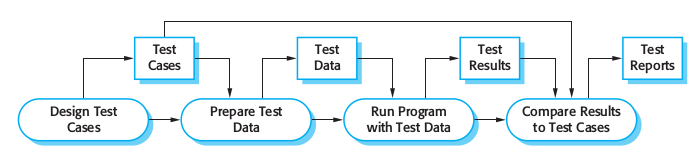
\includegraphics[scale=0.5]{imagens/fig8_3_v.png}
\caption{Modelo do processo de teste de software - essa imagem será trocada}
\label{fig:processo_teste}
\end{figure}

Ainda sobre casos de testes segundo \cite{myers2011art} é de grande importância um bom planeamento, já que é impossível realizar um teste completo. Um boa estratégia é tentar fazer o teste o mais completo possível dada as restrições de tempo e custo. Levando isso em conta a questão-chave se torna: qual o subconjunto de casos de testes entre todos os casos de testes possíveis tem a maior probabilidade de detectar a maior parte das falhas? Em geral, é impraticável, muitas vezes impossível, encontrar todos os erros em um programa. Este problema fundamental, por sua vez, terá implicações para a economia dos testes, os pressupostos que o testador terá que fazer sobre o programa e a maneira como os casos de teste são projetados.

Para encontrar um equilíbrio entre o menor número de casos de testes e uma ótima cobertura do programa são adotadas estratégias de teste de software. Uma estratégia para testes de software fornece um roteiro que descreve as etapas a serem realizadas como parte do teste, quando as etapas são planejadas, realizadas, e quanto esforço, tempo e recursos serão necessários. Portanto, qualquer estratégia de teste deve incorporar o planejamento do teste, a execução do teste e a coleta e avaliação de dados resultantes \cite{pressman2005software}.

Neste trabalho serão apresentadas duas abordagens que são utilizadas para identificar casos de testes, uma é baseada em especificação e é tradicionalmente chamada de testes funcionais, e a baseada em código chamada de testes estruturais \cite{jorgensen2016software}. Os testes funcionais também são conhecidos por teste de caixa preta, estes testes são realizados na interface do software e com pouca consideração à estrutura lógica interna do software. O teste de caixa branca também conhecido como teste estrutural é baseado em uma análise dos detalhes procedurais, os caminhos lógicos através do software e as colaborações entre componentes \cite{pressman2005software}.

\subsection{Teste de caixa preta}

O termo caixa preta é utilizado fazendo referência que o projetista de testes não tem acesso ao código fonte do programa, sendo a parte interna do sistema desconhecida, assim o desenvolvimento do projeto de teste é realizado apenas tendo conhecimento da especificação do software. Para estes testes a única informação utilizada é a especificação do software, portanto os casos de testes são independentes de como o sistema é implementado, não gerando problemas se ocorrerem mudanças na implementação, e o desenvolvimento dos casos de teste podem ocorrer em paralelo com com a implementação \cite{jorgensen2016software}.

De acordo com \cite{pressman2005software} esta abordagem de testes permite que se obtenha conjunto de condições de entradas que exercerão plenamente todos os requisitos funcionais de um programa. As principais de erros encontrados são funções incorretas ou ausentes, erros de interfaces, erros em estruturas de dados ou acesso externo ao banco de dados, erros de comportamento ou desempenho e erros de inicialização e finalização do sistema.

Alguns dos pontos negativos dos testes baseados em especificação são que podem ocorrer redundâncias entre os casos de testes agravada pela possibilidade de partes do software que não foram testadas. E como os teste são baseados no comportamento especificado, é difícil de imaginar esses métodos identificando comportamentos que não são especificados \cite{jorgensen2016software}.

\subsection{Teste de caixa branca}

O nome caixa branca vem da exigência do conhecimento de como o software é implementado, enxergar o seu funcionamento interno, para executar esta técnica, por exemplo o diferentes casos de testes podem ser derivados para um laço de repetição de um código, sendo independente da funcionalidade do software \cite{graham2008foundations}. Usando métodos de caixa branca é possível derivar casos de testes que garantem que todos os caminhos lógicos tenho sido exercidos pelo menos uma vez, como os lados verdadeiros e falso de uma decisão lógica, os laços de repetições e outras estruturas para garantir a sua validade \cite{pressman2005software}. Com os conceitos de teoria de grafo é possível descrever exatamente o que será testado, esta técnica serve também para a definição e uso de métricas de cobertura de teste, indicando até que ponto o software foi testado oferecendo assim um melhor gerenciamento de teste \cite{jorgensen2016software}.

Entre os teste de caixa branca temos o teste de caminho ou \textit{path testing}, onde um programa é derivado(tranformado em) em um grafo direcionado em que os nós são fragmentos de declaração e as ligações chamadas de arestas representam o fluxo de controle. Para derivar um um programa procedural em grafo de fluxo podemos usar a notação da Figura \ref{fig:4estrutura_basica} para cada uma das construções básicas da programação estruturada \cite{jorgensen2016software}.

\begin{figure}[ht]
\centering
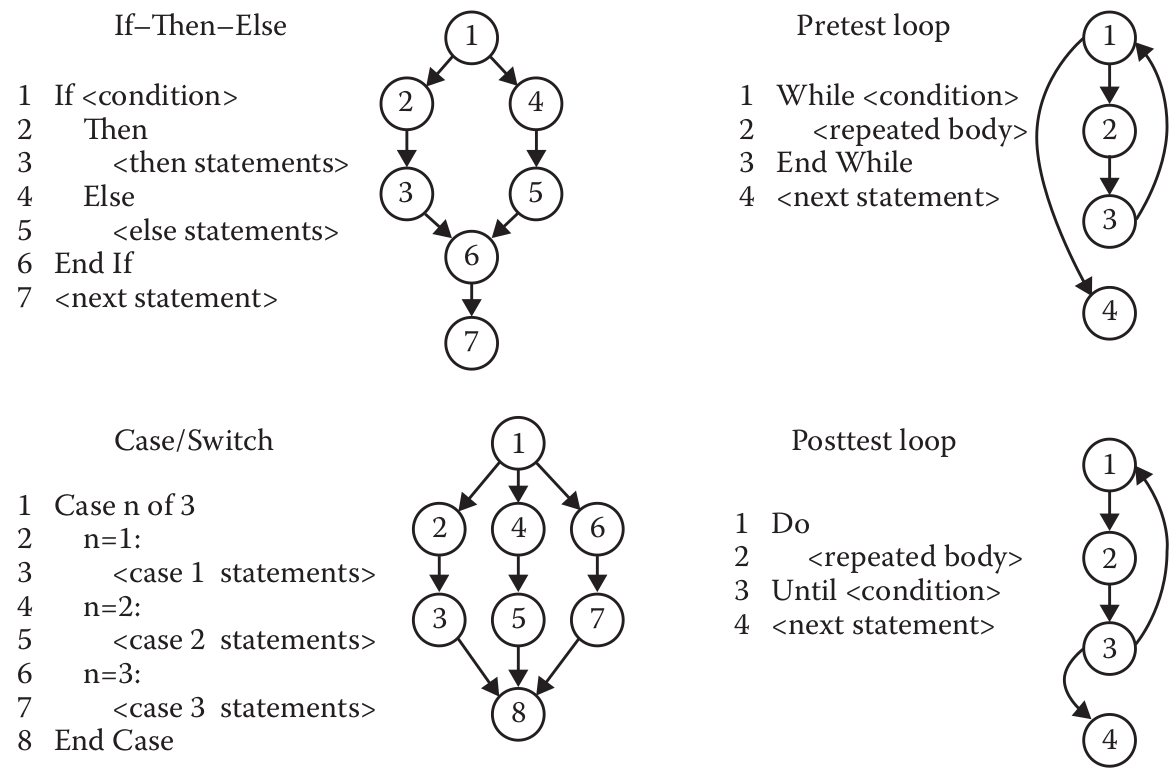
\includegraphics[scale=0.3]{imagens/const_basica_grafo.png}
\caption{Grafos para as quatro estruturas básicas da programação procedural}
\label{fig:4estrutura_basica}
\end{figure}

\cite{jorgensen2016software} define que dado um conjunto de casos de teste para um programa eles constituem a cobertura de nó quando executados no programa cada nó no grafo é percorrido e constituem cobertura de aresta se quando executado no programa, cada aresta do no grafo for percorrida. \cite{winikoff2014testability} em seu trabalho apresenta um exemplo representado na Figura \ref{fig:exemplo_grafo}, onde existem 2 caminhos pelo programa ( 1, 2, 3, 5, 6) e (1, 2, 4, 5, 6). Um conjunto de testes para ser adequado deve ter pelo menos 2 casos de testes, um para exercitar cada caminho possível do programa.

\begin{figure}[ht]
\centering
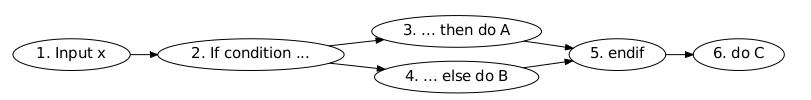
\includegraphics[scale=0.5]{imagens/exemplo_grafo.png}
\caption{Exemplo de grafo de fluxo de um programa}
\label{fig:exemplo_grafo}
\end{figure}


%\subsubsection{Testes evolutivo}

\subsection{Testes de sistemas no ciclo de desenvolvimento de software}

O projeto de testes para um software está diretamente relacionado ao modelo de ciclo escolhido para o desenvolvimento do sistema. Existem vários processos de desenvolvimento de software entre eles, modelo cascata, modelo iterativos, e modelos baseados em metodologias ágeis, eles especificam as várias etapas do processo e a ordem em que são realizadas. A escolha destes depende dos objetivos e metas do sistema a ser desenvolvido, mas sempre levando em conta que a qualidade e confiabilidade são os principais fatores \cite{graham2008foundations}.


Os níveis de teste de software do \textit{V-Model} espelham o modelo cascata do ciclo de vida de desenvolvimento de software. Apesar deste modelo apresentar desvantagens ele é útil para identificar níveis distintos e esclarecer objetivos e responsabilidades para cada nível de teste. Uma variação do modelo cascata é apresentada na Figura \ref{fig:v-model} apresentando os níveis de testes relacionados a cada etapa do desenvolvimento \cite{jorgensen2016software}. 

\begin{figure}[ht]
\centering
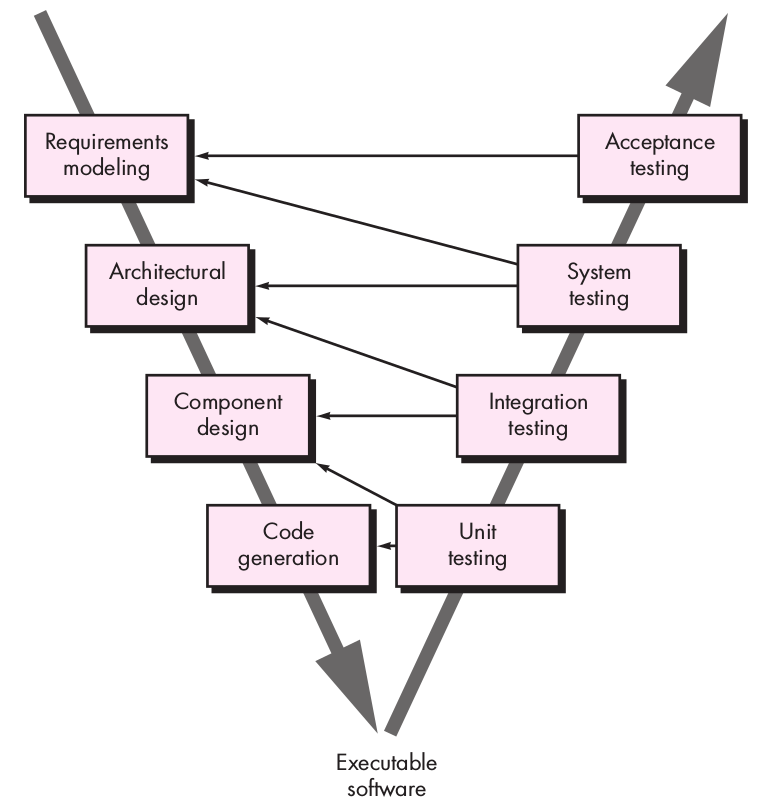
\includegraphics[scale=0.3]{imagens/v-model.png}
\caption{V Model}
\label{fig:v-model}
\end{figure}

A grande contribuição do \textit{V-Model} foi a orientação de que o teste precisa começar o mais cedo possível no desenvolvimento do projeto. As atividades de teste devem ser realizadas em paralelo com as atividades de desenvolvimento, e toda a equipe deve trabalhar juntos para se possa identificar defeitos em decisões de projeto que de outra forma, separadamente, dificilmente seriam percebidas e comunicadas. A identificação precoce de defeitos é, de longe, o melhor meio de reduzir o seu custo final \cite{ammann2016introduction}.

\cite{graham2008foundations,ammann2016introduction} descrevem os níveis dos testes utilizados e seus objetivos:

\begin{itemize}
\item Teste de Aceitação: são projetados para determinar se o software atende aos requisitos e regras de negócio, os testes são realizados com dados fornecidos pelo cliente do sistema e não com dados de teste simulados, e podem revelar erros e omissões na definição de requisitos do sistema, problemas de requisitos onde as instalações do sistema não atendem às necessidades do usuário ou desempenho do sistema inaceitável. Este nível de teste deve envolver o usuário ou alguém com conhecimento do domínio do sistema. 
\item Teste de Sistema: se preocupa com o comportamento do sistema e se ele está em conformidade com os requisitos definidos no projeto. Nesta etapa assume-se que as blocos de software estão funcionando de acordo, pois encontrar uma falha de nível inferior pode ter um grande custo para uma correção. Os testes geralmente são realizados por uma equipe específica para esta tarefa e não pelos programadores.
\item Teste de Integração: projetado para avaliar a interação entre se as interfaces dos módulos funcionam corretamente. É uma técnica sistemática para a construção da arquitetura de software ao mesmo tempo que se investiga erros associados à interface. Uma das abordagens é construir o programa incrementalmente e cuidadosamente incluindo e testando módulos todos os componentes, assim erros são mais fáceis de isolar e corrigir, geralmente é responsabilidade da equipe de desenvolvimento.
\item Teste de Unidade: avalia as unidades produzidas na fase de implementação, é o nível de teste que verifica as menores unidades do software como por exemplo classes, objetos e funções. Os erros encontrados pelos testes são limitados ao escopo estabelecido para o teste unitário, este concentra-se na lógica do processamento interno.  É comum os testes unitários serem empacotados juntamente com o código fonte e serem utilizados para testes automáticos em outros momentos.
\end{itemize}


\section{Teste de Software em SMA}

Os agentes e sistemas multiagentes possuem muitas peculiaridades que tornam o processo de teste mais complexo e que devem abordar algumas questões que não eram preocupação no desenvolvimento de software orientado a objetos. Algumas dessas dificuldades foram citadas em \cite{rouff2002test,houhamdi2011multi,nguyen2009thesis} e são apresentadas a seguir:

\begin{itemize}
\item Distribuído/assíncrono: os agentes podem operar de forma simultânea e assíncrona, ou seja, um agente pode ter que aguardar que outros agentes cumpram seus objetivos que o contexto permita a execução de seus planos. Um agente pode funcionar corretamente isolado, mas incorretamente quando colocado em uma comunidade de agentes ou vice-versa.
\item Autônomos: Os agentes são autônomos, as mesmas entradas de testes podem resultar em comportamentos diferentes em diferentes execuções, uma vez que os agentes podem modificar sua base de conhecimento entre duas execuções ou podem aprender com entradas anteriores.
\item Envio de mensagens: os agentes se comunicam através de envio de mensagens. As técnicas de teste tradicionais, envolvendo chamadas de método, não podem ser aplicadas diretamente.
\item Fatores ambientais e normativos: O ambiente e convenções (normas, regras e leis) são fatores importantes que definem ou influenciam os comportamentos dos agentes. Diferentes configurações do contexto podem afetar os resultados do teste. Ocasionalmente, um contexto dá meios para que os agentes se comuniquem ou em si é uma entrada de teste.
\item Agentes “selados”: Os agentes podem fornecer primitivas observáveis ou não ao mundo exterior, resultando em acesso limitado ao estado e ao conhecimento dos agentes internos. Um exemplo poderia ser um SMA aberto que permite que agentes de terceiros acessem os recursos do SMA, semelhante ao funcionamento de APIs. Nestes casos como garantir que estes agentes de terceiros com o conhecimento limitado sobre suas intenções tenham um comportamento apropriado.
\end{itemize}



%Ainda testar um único agente é diferente de testar uma comunidade de agentes. Ao testar um único agente o foco é na funcionalidade deste agente e se ele opera para um conjunto de mensagens, entradas ambientais e condições de erro. Testar uma comunidade de agentes torna objetivos de testes mais amplos, tendo que verificar se os agentes da comunidade trabalham juntos como projetado, atestando a troca de comunicação entre eles, averiguando se essa troca de mensagem realmente está ocorrendo entre os agentes previstos  e  com o ambiente, mas agora com um agravante de ter um número muito maior de interações \cite{rouff2002test}.

Testar um único agente é diferente de testar uma comunidade de agentes. O teste de agentes pode ser feito incremental durante o desenvolvimento testando funcionalidades à medida que elas são adicionadas. Alguns dos principais erros ao desenvolver agentes podem ser endereçar incorretamente uma mensagem para outro agente, enviar uma solicitação incorreta em uma mensagem ocorrendo que o agente receptor não reconheça a mensagem, analisar incorretamente mensagens recebidas, enviar uma mensagem ao agente errado, ou até mesmo não ter desenvolvido códigos do agente para que ele seja capaz de aceitar todas as mensagens \cite{rouff2002test}. Outros testes a serem realizados é verificar se a comunicação com o ambiente está correta e se a aprendizagem está adequada.

\begin{figure}[ht]
\centering
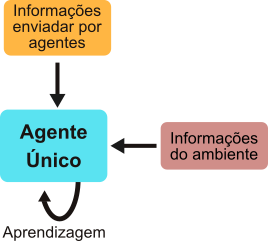
\includegraphics[scale=0.5]{imagens/agente_unico.png}
\caption{Teste em um Agente}
\label{single}
\end{figure}

Testar uma comunidade de agentes torna os objetivos de testes mais amplos, tendo que verificar se os agentes da comunidade trabalham juntos como projetado, atestando a troca de comunicação entre eles, averiguando se essa troca de mensagem realmente está ocorrendo entre os agentes previstos  e  com o ambiente, mas agora com um agravante de ter um número muito maior de interações. \cite{rouff2002test} cita os erros mais observados em programadores desenvolvendo comunidades de agentes.

\begin{figure}[ht]
\centering
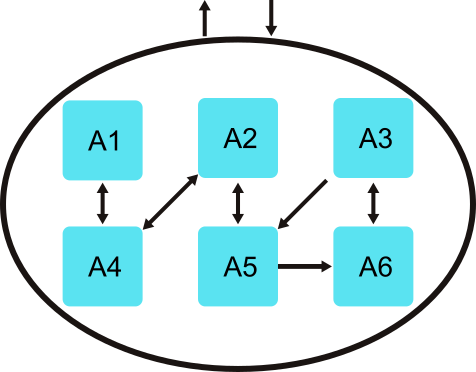
\includegraphics[scale=0.5]{imagens/agente_comunidade.png}
\caption{Teste em comunidade de agentes}
\label{comunity}
\end{figure}

\begin{itemize}
\item Não documentar adequadamente as interações do agente, de modo que desenvolvedores diferentes implementam as interações de forma diferente
\item Erro na mensagem, não comunicando o remetente, o conteúdo, entre outros, nas mensagens do agente
\item Projetando impasses nas trocas de mensagens
\item Não implementando mudanças nas mensagens para todos os agentes ao mesmo tempo (o que dificulta o teste da comunidade).
\end{itemize}

Para uma melhor organização dos testes em agentes, assim como os testes no ciclo de vida de desenvolvimento de software tradicional os testes nos SMA também possuem vários níveis. O teste de unidade possui o mesmo nome nas duas abordagens, o segundo nível é o teste de agente não possui um relacionado. O teste de  grupo se relaciona com o teste de integração, o teste de sociedade está relacionado com o teste de sistema. E por último e com o mesmo nome tem o teste de aceitação \cite{houhamdi2011multi}. 

Os testes de unidade certificam-se que os menores unidades que compõem o agente estejam funcionando de acordo com o que foi planejado, Essas unidades incluem os blocos de código que implementam as metas, planos, base de conhecimento, mecanismos de raciocínio, especificação de regras entre outros. Já os testes de agentes testa a integração destas pequenas unidades de dentro do agente, verificando se os agentes são capazes de cumprir suas metas e se interagem corretamente com o ambiente. O teste de grupo avalia a interação entre agentes, protocolo de comunicação e semântica, integração com o ambiente, integração de agentes com recursos compartilhados, observa propriedades emergentes e comportamentos coletivos, este teste certifica que um grupo de agentes e o ambiente funcionem corretamente juntos. O teste de sociedade testa o SMA em execução no ambiente operacional de destino, testa as propriedades emergentes e macroscópicas esperadas do sistema. E o teste de aceitação testa o SMA no ambiente de execução do cliente e verifica se ele atende aos objetivos esperados das partes interessadas \cite{nguyen2009thesis}.

\section{Sistemas Multiagentes}

  Bla blabla blablabla bla.  Bla blabla blablabla bla.  Bla blabla blablabla


\subsection{Agente}

  Bla blabla blablabla bla.  Bla blabla blablabla bla.  Bla blabla blablabla


\subsection{Ambiente}

  Bla blabla blablabla bla.  Bla blabla blablabla bla.  Bla blabla blablabla


\subsection{Organização}

  Na nossa sociedade temos diversas organizações, o que se mostrou uma maneira eficaz de coordenar comportamentos. A organização de um sistema multi-agente é a coleção de papéis, relacionamentos e estruturas de autoridade que regem seu comportamento. Geralmente os SMA têm alguma forma de organização, embora possa ser implícita e informal. As organizações de agentes orientam o modo como os membros da população interagem uns com os outros, não necessariamente num dado momento a momento, mas sim a longo prazo.Essa orientação pode influenciar as relações de autoridade, fluxo de dados, alocação de recursos, padrões de coordenação ou qualquer outra série de características do sistema \cite{horling2004survey}.

Existem vários modelos de organizações e eles estruturam o comportamento de entidades complexas em uma hierarquia de entidades encapsuladas onde cada membro tem funções a desempenhar. As funções ou papéis (nesta dissertação será adotado papel para a tradução de \textit{role}) estruturam os departamentos, e estes estruturam uma organização. A teoria da organização analisa como estas organizações funcionam, suas principais características, as características mais relevantes dos membros, os papéis gerais que os membros adotam, os relacionamentos entre os membros, a hierarquia, as regras e normas que regem a organização , etc\cite{argente2006multi}. Isso pode ajudar grupos de agentes simples a exibir comportamentos complexos e ajudar agentes sofisticados a reduzir a complexidade de seus raciocínios. Implícito neste conceito é o pressuposto de que a organização tem algum propósito - que a forma, o tamanho e as características da estrutura organizacional podem afetar o comportamento do sistema \cite{horling2004survey}.

\cite{malone1994interdisciplinary} define coordenação como gestão de dependências entre atividades independentes. Esta definição para coordenação tem um sentido inclusivo para diferentes áreas de conhecimento, podendo ser aplicado em teoria organizacional, economia, ciência política, biologia, entre outros. Para a computação as dependências entre diferentes processos computacionais se assemelham a interações entre pessoas, e devem ser estudados como podem ser gerenciadas.

Organização baseado na administração apresenta duas abordagens diferentes \cite{boella2006coordination}: 

\begin{itemize}
\item organizações cujo objetivo é gerar serviços, produzir bens (fábricas, empresas de serviços) ou causar certos efeitos no meio ambiente (por exemplo, autoridades Polícia, partidos políticos, grupos de interesse, sindicatos, etc.) 
\item organizações cujo objetivo é mudar indivíduos (por exemplo, escolas, universidades, hospitais, prisões).
\end{itemize}

No início os sistemas tinham apenas uma visão mais centrada nos aspectos individuais dos agentes de modo que o SMA é projetado em termos de estados mentais deste, como as crenças, intenções, objetivos, etc conhecida como metodologia orientada a agentes. Apartir daí os SMA evoluíram para a metodologia orientada para a organização, levando em conta seus principais objetivos, estrutura e normas sociais\cite{argente2006multi}. 

Duas tendências diferentes podem ser observadas ao comparar várias abordagens. Por um lado, métodos detalham funções, grupos e relacionamentos do sistema, mas não explicitamente considere as normas sociais. Por outro lado, métodos e estruturas como estão focadas nas normas sociais e explicitamente definir políticas de controle para estabelecê-las e reforçá-las. O principal objetivo desses métodos é o design de sistemas multiagentes abertos, nos quais agentes com comportamento auto-interessado podem participar. Esses agentes podem ser controlados por meio de normas sociais e uma estrutura organizacional adequada\cite{argente2006multi}.

Os modelos de organização tornaram-se populares para coordenar entidades autônomas em sistemas abertos, descentralizados e dinâmicos como as tecnologias SMA. Estes modelos propõem uma regulação dos SMA por um conjunto de normas, planos, mecanismos e/ou estruturas formalmente especificadas para alcançar algum objetivo global desejado.

Um modelo representa a realidade para o propósito dado, sendo uma abstração da realidade no sentido de que ela não pode representar todos os aspectos da realidade. Isso nos permite lidar com o mundo de forma simplificada, evitando a complexidade, o perigo e a irreversibilidade da realidade \cite{rothenberg1989nature}. Um sistema pode ser representado por um conjunto de modelos diferentes, onde um modelo captura um aspecto específico do sistema, dependendo da finalidade desse modelo específico.

Um modelo organizacional consiste em uma estrutura conceitual e uma sintaxe em que as especificações para organizações de agentes podem ser escritas. A partir destas especificações uma organização pode ser editada em uma plataforma SMA, ou então pode ser utilizado infraestruturas de gerenciamento de organização, que possuem as especificações para que um agente possa saber como acessar os serviços, e fazer solicitações de acordo com o modelo organizacional disponível, podendo assim fazer parte de uma organização.

Os modelos de organização podem ainda dar origem a metamodelos de organização. Um metamodelo representa uma sintaxe abstrata de uma linguagem de modelagem \cite{steinberg2008emf}. Os meta-modelos são usados para produzir e definir especificações de organização e as especificações da organização são usadas para implementar organizações.

A seguir, descreveremos diferentes abordagens baseadas em metamodelos existentes para organizações de modelagem em SMA.

\section{Engenharia de Software Orientada a Agentes}

A Engenharia de Software Orientada a Agentes (AOSE), está preocupada com a forma de engenharia efetiva de sistemas de agentes, isto é, como especificar, projetar, implementar, verificar e manter estes softwares \citep{winikoff2009future}. \citep{sturm2014agent} apresenta as áreas de atuação da AOSE representada pela Figura \ref{fig:aose_areas}.

\begin{figure}[ht]
\centering
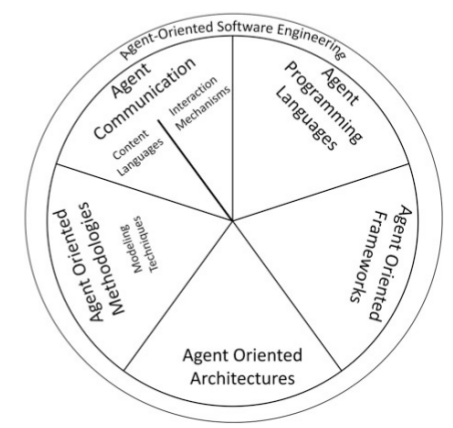
\includegraphics[scale=0.5]{imagens/aose_areas.png}
\caption{Atuação da AOSE}
\label{fig:aose_areas}
\end{figure}

\subsection{Metodologias AOSE}

Segundo \citep{padgham2016agent} muitos autores veem os agentes de software como uma evolução dos objetos promovendo uma abstração e encapsulamento, e deste modo ocorreram tentativas de desenvolver metodologias para o desenvolvimento de software baseado em agentes aproveitando técnicas da engenharia de software tradicional. 

Para \citet{akbari2010survey} uma metodologia de engenharia de software orientada por agente é um processo comercial de desenvolvimento de software, equipado com conceitos distintos e ferramentas de modelagem, nas quais a chave é a abstração usada em seus conceitos que é a de um agente. Apesar de AOSE já existir pelo menos há duas décadas muito ainda tem a ser feito para uma adoção maior da industria. Alguns pontos a serem melhorados \cite{sturm2014agent}:

\begin{itemize}
\item Definição de um conjunto central de propriedades dos agentes.
\item Esclarecer como a AOSE pode facilitar o gerenciamento da complexidade na Engenharia de Software.
\item Padronização das técnicas de AOSE já desenvolvidas
\item Maior integração de tecnologia multi-agentes com as tecnologias já utilizadas na industria.
\end{itemize}

Além desses pontos que exigem uma grande atenção para uma maior adoção do mercado, \citet{sturm2014landscape} reforça que as metodologias orientadas a agentes atuais focam seus esforços no desenvolvimento de novos sistemas e não nos outros estágios e aspectos de ciclo de vida do sistema, como são compreendidos na engenharia de software tradicional. O teste de software e o aspecto de manutenção do sistema dificilmente são suportado dentro das metodologias orientada a agentes.

\begin{table}[h]
\centering
\caption{Metodologias AOSE}
\label{tab:metodologias}
\begin{tabular}{@{}lll@{}}
\toprule
Nome da Metodologia & Ano de Origem & Domínio de Origem \\ \midrule
ADELFE              & 2002          & ES                \\ 
GAIA                & 2000          & ES                \\ 
INGENIAS            & 2002          & ES                \\ 
MaSE                & 1999          & ES                \\ 
MESSAGE             & 2000          & ES                \\ 
Prometheus          & 2002          & ES + IA-EC        \\ 
Tropos              & 2001          & ES+ IA-EC         \\ \bottomrule
\end{tabular}
\end{table}
  
\subsubsection{Moise}

\section{Trabalhos Relacionados}

\subsection{On the Testability of BDI Agent Systems}

Em \cite{winikoff2014testability} o objetivo é avaliar o quão difícil é testar um programa de agente na arquitetura BDI. Para isso é utilizado a técnica de caixa-branca que são baseados no fluxo de controle, um critério básico e muito longo para avaliar a adequação de um conjunto de testes em que todos os caminhos (\textit{All-Path}) do programa sejam cobertos. Um motivo pela escolha de utilizar todos os caminhos é que os SMA geralmente envolvem ambientes não-episódicos, sendo que o comportamento de um determinado plano ou meta é geralmente sensível ao histórico do agente, precisando assim considerar as diferentes histórias possíveis.

Neste trabalho pala analisar o processo de execução BDI é utilizada uma visão declarativa. Os eventos e planos podem ser visualizados como uma árvore em que cada objetivo tem como filhos as instâncias do plano que são aplicáveis a ele, e cada instância do plano tem como filhos os sub-objetivos que ele publica. Esta forma de visualização facilita a análise do número de caminhos através de um programa BDI.

Para a geração de árvore um programa em Prolog foi implementado, onde uma árvore de plano-meta é representada por termos Prolog com a gramática apresentada na Figura \ref{fig:prolog} onde árvore de plano-meta (Goal-Plan Tree) é representado por GPT, o AoGL abreviou lista de ação ou meta (Action or Goal List) e A é um símbolo. Por exemplo a Figura \ref{fig:arvore} mostra a árvore de plano-meta simplificada modelada pelo termo Prolog \begin{math} goal\left ( \left [ plan\left ( \left [ act\left ( a \right ) \right ] \right ),plan\left ( \left [ act\left ( b \right ) \right ] \right ) \right ] \right )\end{math}.

\begin{figure}
  \centering
  \subfigure[Prolog]{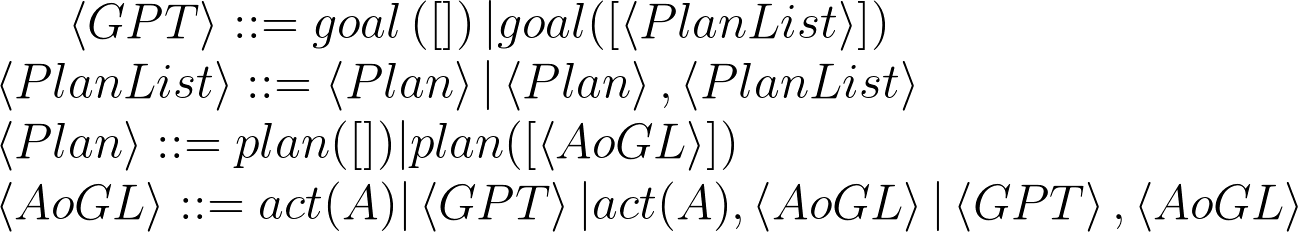
\includegraphics[width=0.6\textwidth]{imagens/code.png}\label{fig:prolog}}
  \subfigure[Árvore]{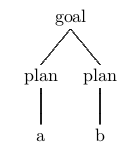
\includegraphics[width=0.2\textwidth]{imagens/simple_tree.png}\label{fig:arvore}}
  \caption{COLOCAR UMA CAPTION AQUI}
  \label{fig:prolog,arvore}
\end{figure}

Com isso em vez de ver a execução de um programa BDI como um processo, o programa é visualizado como uma transformação de dados de uma árvore de planos-metas (finita) em uma sequencia de execuções de ações. Assim, a questão de quão grande é o espaço de comportamento para os agentes BDI é respondida derivando fórmulas que permitem calcular o número de comportamentos, bem-sucedidos e mal sucedidos (ou seja, falhou) para uma determinada planta de plano de meta.

Após testes em modelos de execução BDI abstratos os autores verificaram se os dados obtidos se aplicavam também à modelos reais. A aplicação real escolhida foi o trabalho de \cite{burmeister2008bdi} que preenchia os requisitos para a comparação. Os valores obtidos são apresentados na Tabela \ref{tab:result_ontestability} onde $n^{\checkmark}(g)$ são os caminhos que os testes são bem sucedidos, $n^{\upchi}(g)$ são os caminhos onde os teste falham e $\ell$ são ações antes, depois e entre sub-metas em um plano.

% Please add the following required packages to your document preamble:
% \usepackage{booktabs}
% \usepackage{multirow}
\begin{table}[ht]
\centering
\caption{Resultado do teste realizado em uma aplicação BDI}
\label{tab:result_ontestability}
\begin{tabular}{@{}lllll@{}}
\toprule
\multirow{2}{*}{Workflow with 57 goals} & \multicolumn{2}{l}{Sem manipulação de Falha} & \multicolumn{2}{l}{Com manipulação de Falha}                  \\
                                        & $n^{\checkmark}(g)$     & $n^{\upchi}(g)$    & $n^{\checkmark}(g)$           & $n^{\upchi}(g)$               \\ \midrule
$\ell = 4$                              & 294,912                 & 3,250,604          & $\approx 2.98 \times 10^{20}$ & $\approx 9.69 \times 10^{20}$ \\
$\ell = 2$                              & 294,912                 & 1,625,302          & $\approx 6.28 \times 10^{15}$ & $\approx 8.96 \times 10^{15}$ \\
$\ell = 1$                              & 294,912                 & 812,651            & $\approx 9.66 \times 10^{11}$ & $\approx 6.27 \times 10^{11}$ \\ \bottomrule
\end{tabular}
\end{table}

Neste artigo os autores concluíram que um teste completo em um sistema BDI não é viável. O tamanho de espaços de comportamento é muito grande e ainda se torna significativamente maior quando o sistema tem suporte à manipulação de falhas. Os autores também chegaram à conclusão de que o mecanismo de recuperação de falhas é eficaz para alcançar uma baixa taxa de falha real. E novas abordagens foram propostas para lidar com a testabilidade do sistema.

\subsection{BDI agent testability revisited}

O trabalho \cite{winikoff2017bdi} volta com o objetivo de avaliar se é possível obter garantias em um sistema multiagente através de testes, verificando a testabilidade de um programa, dando continuidade no trabalho anterior \cite{winikoff2014testability}, mas utilizando novas métricas. A testabilidade de um programa é um métrica que indica o esforço necessário para testar adequadamente um programa. Este trabalho tem por objetivo quantificar quantos testes são necessários para testar um um programa de agente BDI para satisfazer um critério considerando o critério de adequação do teste de todas as arestas, que é considerado como o mínimo geralmente aceito \cite{jorgensen2016software}. 

Uma das grandes contribuições dos autores é que a  análise é genérica permitindo a aplicação a todos os programas que utilizam a arquitetura BDI. Para esta análise equações são derivadas  para chegar a conclusão de quantos casos de teste (caminhos) são necessários para cobrir todas as arestas no gráfico de fluxo de controle correspondente a um determinado programa BDI.

A Figura \ref{fig:control_fluxo} apresenta um exemplo de um grafo de controle de fluxo de um programa BDI, este programa tem início em “S” e possui quatro ações $\alpha_{1}, \alpha_{2}, \alpha_{3}$ e $\alpha_{4}$. Caso alguma das ações forem bem-sucedidas então o programa executa “Y” e é encerrado em “E” concluindo-se com sucesso. Se a ação $\alpha_{1}$ falhar ela avança para ação $\alpha_{2}$ que pode ter sucesso ou a falha pode ocorrer novamente e assim a próxima ação seria executada. Este programa exigiria 5 testes para cobrir todas as bordas, um teste é onde as quatro ações falham ($S \rightarrow \alpha_{1} \rightarrow \alpha_{2} \rightarrow \alpha_{3} \rightarrow \alpha_{4} \rightarrow N \rightarrow E$) e os outros 4 testes é para quando uma ação é bem-sucedida e a anterior falhou.

\begin{figure}[ht]
\centering
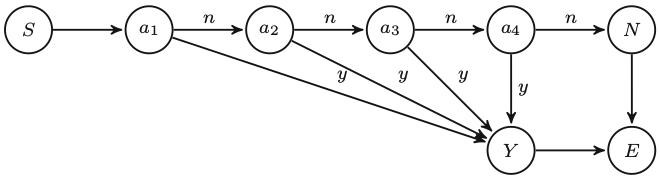
\includegraphics[scale=0.5]{imagens/control_flow.png}
\caption{Controle de Fluxo}
\label{fig:control_fluxo}
\end{figure}

Para derivar equações que calculem o menor número de caminhos exigidos de um programa começando em $S$ para chegar em $E$ é necessário descobrir quantos destes caminhos são bem-sucedidos (passando por $Y$) e quantos falharam (passando por $N$). Os autores definiram $p(P)$ como o número de caminhos necessários para cobrir todas as arestas do grafo de fluxo de controle correspondente ao programa $P$, $y(P)$ para os caminhos que vão por $Y$ e $n(P)$ para os caminhos que vão por $N$, então $p(P) = y(P) + n(P)$.

Logo após os autores consideram $P_{1};P_{2}$, onde um subprograma $P_{1}$ é colocado em sequencia com $P_{2}$ Figura \ref{fig:grafop1p2}. O subprograma $P_{1}$ requer $p(P_{1})$ testes para cobrir todas as arestas com $n(P_{1})$ testes levando até a falha e $y(P_{1})$ levando à uma execução com sucesso.

\begin{figure}[ht]
\centering
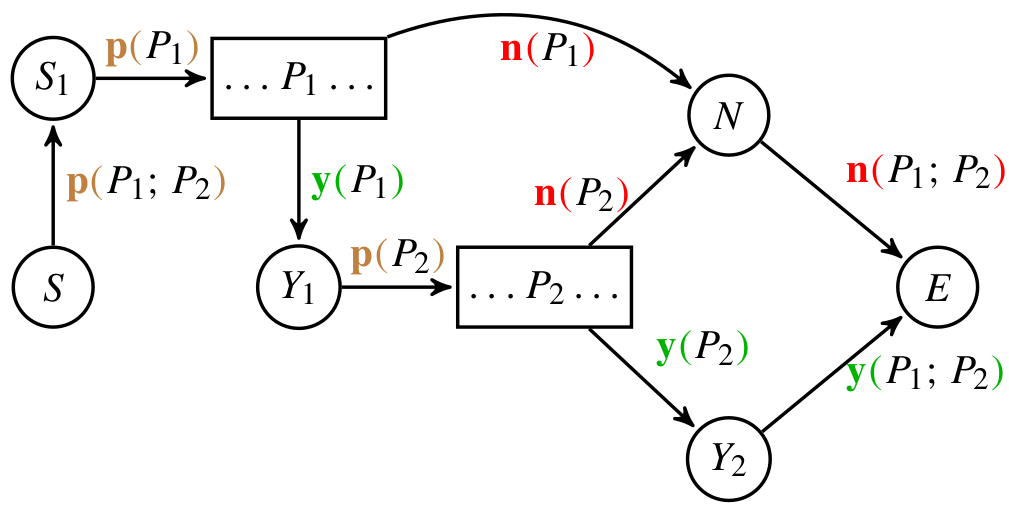
\includegraphics[scale=0.3]{imagens/grafop1p2.png}
\caption{Controle de Fluxo de $P_{1};P_{2}$}
\label{fig:grafop1p2}
\end{figure}

A partir do exemplo da Figura \ref{fig:grafop1p2} diversas equações são derivadas para os diferentes casos. Estas equações servem para determinar quantos testes são necessários para garantir uma cobertura adequada em relação ao critério todas as arestas. Então os autores implementam as equação em um programa Prolog que calcula os valores de p(p), y(P) e n(P) para qualquer programa BDI. A Tabela \ref{tab:bdirevisited} contém a comparação dos resultados do trabalho anterior dos autores \cite{winikoff2014testability} com os novos resultados encontrados.

\begin{table}[ht]
\begin{threeparttable}
\centering
\caption{Comparação entre os resultados dos trabalhos \cite{winikoff2014testability,winikoff2017bdi}}
\label{tab:bdirevisited}
\begin{tabular}{lllllll}
\hline
                   & \multicolumn{2}{c}{Todos Caminhos}                                            & \multicolumn{4}{c}{Todas Arestas}                             \\ \cmidrule(l){2-7} 
d = j = k = 3      & \multicolumn{1}{c}{n$^{\checkmark}$(g)} & \multicolumn{1}{c}{n$^{\upchi}$(g)} & \multicolumn{2}{c}{p(\textg)} & \multicolumn{2}{c}{p(\cancel{\textg})} \\ \cline{4-7} 
                   &                                         &                                     & Rel.           & Aplic.       & Rel.          & Aplic.        \\ \hline
62 (j = k = 2)     & $6.33 \times 10^{12}$                   & $1.82 \times 10^{13}$               & $141$          & $78$         & $85$          & $64$          \\
363                & $1.02 \times 10^{107}$                  & $2.56 \times 10^{107}$              & $6391$         & $2961$       & $469$         & $378$         \\
776 (j = 2, d = 4) & $ 1.82 \times 10^{157}$                 & $7.23 \times 10^{157}$              & $1585$         & $808$        & $1037$        & $778$         \\
627 (k = 4)        & $3.13 \times 10^{184}$                  & $7.82 \times 10^{184}$              & $10,777$       & $4767$       & $799$         & $642$         \\ \bottomrule
\end{tabular}
    \begin{tablenotes}
      \small
      \item This is where authors provide additional information about
      the data, including whatever notes are needed.
    \end{tablenotes}
    \end{threeparttable}
\end{table}


\chapter{Metodologia}

  Bla blabla blablabla bla.  Bla blabla blablabla bla.  Bla blabla blablabla



\chapter{Conclusão}

  Bla blabla blablabla bla.  Bla blabla blablabla bla.  Bla blabla blablabla
  
\chapter{Cronograma}

\begin{table}[ht]
\centering
\caption{My caption}
\label{my-label}
\begin{tabular}{|l|c|c|c|c|c|c|c|}
\hline
\multicolumn{1}{|c|}{Cronograma}                &                          &                          &                          &                          &                          &                          &                          \\ \hline
                                                & \multicolumn{1}{l|}{Out} & \multicolumn{1}{l|}{Nov} & \multicolumn{1}{l|}{Dez} & \multicolumn{1}{l|}{Jan} & \multicolumn{1}{l|}{Fev} & \multicolumn{1}{l|}{Mar} & \multicolumn{1}{l|}{Abr} \\ \hline
Qualificação                                    & x                        &                          &                          &                          &                          &                          &                          \\ \hline
Desenvolvimento dos Jogos                       & x                        & x                        & x                        &                          &                          &                          &                          \\ \hline
Integração das Ferramentas                      & x                        & x                        & x                        & x                        &                          &                          &                          \\ \hline
Testes com Usuários                             &                          &                          &                          & x                        & x                        & x                        &                          \\ \hline
Análise dos Resultados                          &                          &                          &                          &                          &                          & x                        & x                        \\ \hline
Escrita Dissertação                             & x                        & x                        & x                        & x                        & x                        & x                        & x                        \\ \hline
Escrita de um Artigo com Resultados da Pesquisa &                          &                          &                          &                          &                          & x                        & x                        \\ \hline
Defesa Mestrado                                 &                          &                          &                          &                          &                          &                          &                          \\ \hline
\end{tabular}
\end{table}

% Bibliografia
% http://liinwww.ira.uka.de/bibliography/index.html
% um site que cataloga no formato bibtex a bibliografia em computacao
%\bibliography{nomedoarquivo.bib} (sem extensao)
%\bibliographystyle{formato.bst} (sem extensao)


\bibliographystyle{abnt}
\bibliography{bibliografia}


% Anexos (Opcional)
%\annex
%\chapter{Um Anexo}



\end{document}

